\section{Anforderungsspezifikation}
\subsection{Use Case}
\subsubsection{Aktoren und Stakeholder}
\begin{table}[H]
\centering
    \begin{tabular}{|p{3cm}|p{9cm}|}
    \hline
    \rowcolor{lightblue}
    Aktor & Tätigkeit   \\ \hline
	User  & Startet CrosswalkDetector mit Bounding Box als Eingabeparameter \\ \hline
	CrosswalkDetector & Erkennt Fussgängerstreifen \\ \hline 
	TileProvider & Stellt Orthofotos für die Erkennung der Fussgängerstreifen zu Verfügung.\\ \hline
	OSMProvider & Stellt Strassen - und Fussgängersteifen Informationen zur Verfügung. \\ \hline
	JSON File & Speicherort für die Positionen der ermittelten Fussgängersteifen und deren Strassenzugehörigkeit.\\ \hline
    \end{tabular}
    \caption[Aktoren und Stakeholder]{Aktoren und Stakeholder}
\end{table}

\subsubsection{Use Case Diagramm}
\begin{figure}[H]
\centering
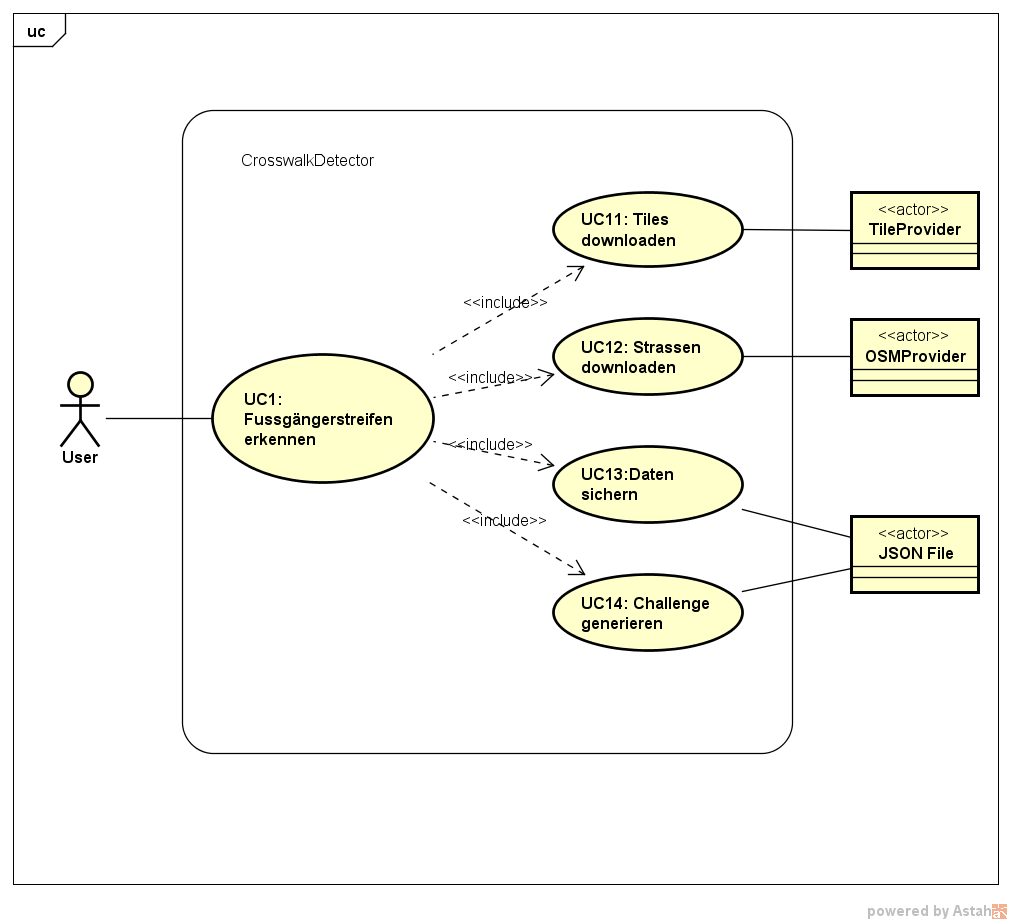
\includegraphics[width=420pt]{images/UseCase.png}
\caption[Use Case Diagramm]{Use Case Diagramm}
\end{figure}

\subsubsection{Use Cases Brief}
\paragraph{UC1: Fussgängerstreifen erkennen}
Der User startet die Applikation und gibt als Eingabeparameter ein Boundingbox an, welche nach Fussgängerstreifen durchsucht wird. Dabei werden Orthofotos mit Hilfe eines Erkennungsalgortithmus abgearbeitet.

\paragraph{UC11: Tiles downloaden} 
Ein TileProvider stellt Orthofotos zur Verfügung, welche herunter geladen werden müssen. Diese werden im Anschluss dem Erkennungsalgorithmus zur Verfügung gestellt.

\paragraph{UC12: Stassen downloaden}
Ein OSMProvider stellt Informationen zu Strassen und Fussgängerstreifen zur Verfügung, welche vom Erkennungsalgorithmus genutzt werden. Mit diesen Daten kann die Suche präzisiert werden, sowie der Download von Orthofotos reduziert werden.

\paragraph{UC13: Daten sichern}
Die Erkannten Fussgängerstreifen werden in einem JSON File persistiert. Dabei sind die Position (Koordinate lat/lon) relevant.

\paragraph{UC14: Challenge generieren}
Mit Hilfe der persistieren Daten wird ein Challenge generiert, welche die Daten über eine Crowdsourcing-System in OpenStreetMap integriert.

\subsubsection{Use Cases Fully Dressed}
\begin{table}[H]
    \begin{tabular}{ | p{4cm} | p{10cm}  | }
    \hline
    Scope & CrosswalkDetection System   \\ \hline
	Level  & User Goal \\ \hline
	Primary Actor & User \\ \hline 
	Stakeholders & 
	\begin{itemize}
		\item System: Möglichst alle Fussgängerstreifen erkennen
		\item User: Einmal gestartet, läuft alles autonom
    \end{itemize} \\ \hline
	Preconditions & 
		\begin{itemize}
		\item User muss Boundingbox bestimmen
		\item OSMProvider muss verfügbar sein
		\item TileProvider muss verfügbar sein
    \end{itemize} \\ \hline
	Postconditions & Koordinaten der Fussgängerstreifen persistiert \\ \hline
	Main Success Scenario & 
	\begin{enumerate}
		\item CrosswalkDetection wird mit Angabe der Boundingbox aufgerufen
		\item Daten von OSMProvider werden heruntergeladen
		\item Orthofotos von TileProvider werden heruntergeladen
		\item Erkennungsalgorithums erfasst Fussgängerstreifen
		\item Daten sind persistiert
	\end{enumerate} \\ \hline
	Extensions & 
	\begin{enumerate}
		\item a) Boundingbox wird aufgeteilt für Parallelisierung
		\item b) Nur Informationen für Strassen und Fussgängerstreifen sind relevant
		\item b) Nur Orthofotos, welche Strassen beinhalten sind werden heruntergeladen
	\end{enumerate} \\ \hline
	Special Requirements & Benutzer soll gut geführt werden und bei Unklarheiten bei
Eingabefeldern Informationen erhalten.
Das Hindernis um sich zu registrieren sollte möglichst klein sein. \\ \hline
	Frequency of Occurrence & Der Vorgang darf beliebig oft wiederholt werden. \\ \hline
	Open Issues & Falls ein Unterbruch statt findet, soll von diesem Zustand weiter gearbeitet werden. \\ \hline
    \end{tabular}
    \caption[Use Case Fully Dressed]{Use Case Fully Dressed}
\end{table}


